% !TEX encoding = UTF-8 Unicode
\documentclass{article}
\usepackage[backend=biber]{biblatex}
\addbibresource{bibliography.bib}
\usepackage[utf8]{inputenc}
\usepackage{amsmath,amssymb}
\usepackage{paralist}
\usepackage{color}
\usepackage[detect-weight=true, binary-units=true]{siunitx}
\usepackage{pgfplots}
\usepackage{authblk}
\usepackage{url}
\usepackage{multirow}
\usepackage{booktabs}

\addtolength{\oddsidemargin}{-.875in}
\addtolength{\evensidemargin}{-.875in}
\addtolength{\textwidth}{1.75in}

\addtolength{\topmargin}{-.875in}
\addtolength{\textheight}{1.75in}

\title{Machine Learning and Data Mining progetto:\\Black Friday}
\author{Michele Belletti}

\date{Corso AA 2019-2020}



\begin{document}

\maketitle



\section{Identificazione del problema}
Questo articolo ha due principali obiettivi:
Il primo è di confrontare  i risultati di diversi algoritmi per identificare quale sia il migliore per la determinazione della qunatità spesa da un utente durante l'evento del Black Friday usando i dati a disposizione \cite{data} . In questo caso abbiamo anche dimostrato come, dopo un analisi dei dati e una loro manipolazione in base alle conoscenza che si riescono ad ottenere dopo l'analisi, possa modificare la stima.
Questo tipo di stimatore permette ad una azienda di fare una stima dei guadagni durante questi tipo di eventi il che puo essere utilizzato per incrementare gli introiti e valutare bene la spesa che l'azienda possa mettere in atto per incentivare l'affluenza.

il secondo è quello di confrontare due algoritmi di classificazione per determinare quale categoria del prodotto esso ha acquistato. Questo modello così realizzato permette una migliore gestione del magazzino perchè fornisce un idea delle abitudine degli utenti inscritti, inoltre permette di creare pubblicità più mirate ad un utente in modo da aumentare gli utili dell'azienda. 


\section{Indici di valutazione e prestazione}
Per la realizzazione dei modelli di stima della quantità dei soldi spesi e del tipo di categoria che un utente compra sono stati utilizzati gli algoritmi della libreria python: scikit-learn \cite{scikit-learn} .
I sistemi di valutazione che abbiamo adottato per questo articolo sono, per la determinazione della quantità di soldi spesi, un confronto sul valore RMSE mentre per la stima del tipo di categoria del prodotto abbiamo utilizzato un indicazione percentuale del corretto individuamento della categoria del prodotto.
Per tale verifica abbiamo utilizzato l'80 \% dei dati a disposizione per la realizzazione del modello mentre il rimanente 20\% per la verifica.

\section{Soluzione Proposta}
Gli algoritmi utilizzati per la creazione dello stimatore della quantità di soldi spesi da un utente sono: regressione lineare, decision tree regression e random forest regression.
L'analisi dei dati ha riportato la presenza di informazioni mancanti (value NaN) nelle categorie dei prodotti 2 e 3. Questo tipo di informazione, data la mancanza di documentazione a riguardo, ci ha portato alla realizzazione di due modelli costruiti usando i dati nei seguenti modi:
\begin{itemize}
\item per il primo metodo abbiamo optato per la diretta eliminazione delle categorie 2 e 3, ipotizzando che contengano informazioni riguardanti alla sottocategoria del prodotto, cioè descrizioni del prodotto di rilievo minore rispetto alla categoria principale;
\item per il secondo metodo abbiamo assegnato una variabile scorrelata (fillna(-2.0) (le altre variabili sono maggiori di 0) ai dati presenti nelle categorie 2 e 3, in modo tale che la sua presenza non fornisca delle informazioni erronee e possa deteriorare il modello. Inoltre aggiungeremo informazioni ricavate dopo l'analisi dei dati, che costituiscono in variabili che definiscono la quantità di operazioni di quel tipo, come spiegato nella sezione successiva.
\end{itemize}

Ottenuti i risultati di questi due metodi abbiamo optato nell'utilizzo dei dati nel secondo caso per la creazione dell'algortmo che determina il prodotto che un utente ha acquistato durante il Black Friday· Gli algoritmi della libreria che abbiamo utilizzato sono Decision Tree Classifier e  Random Forest Classifier.

\section{Valutazione sperimentale}
Per la realizzazione del migliore modello predittivo è necessaria un analisi dei dati a disposizione. Il che come verrà dimostrato permette una migliore stima  del modello.

\subsection{Data}
Come anticipato, i dati a nostra disposizione sono gli ordini effettuati durante il Black Friday e sono costituiti da queste informazioni:
\begin{itemize}
\item L'utente attraverso il suo codice identificativo UserID;
\item Il prodotto che l'utente ha comprato ProductID;
\item L'eta dell'utente: Gender Age (valore che viene diviso ad intervalli di età 0-17, 18-25, 26-35, 36-45, 46-55, 55+;
\item Il tipo di occupazione: Occupation (21 diverse occupazioni);
\item La categoria della città:  CityCategory (A,B,C che si suppone dipendano dalle dimensioni);
\item Quanti anni sono passati da quando vive in quella città: StayInCurrentCityYears (0, 1, 2, 3, 4+);
\item Stato civile: MaritalStatus;
\item Le categorie del prodotto comprato: ProductCategory1, ProductCategory2, ProductCategory3;
\item E la quantità dei soldi spesi: Purchase.
\end{itemize}

Analizzando, con l'ausilio dei grafici sotto riportati (grafici 1-2-3-4-5-6), che rappresentano ogni variabile rispetto al numero di ordini effettuati dai clienti si nota che :

\begin{itemize}
\item persone di età tra i 26-35 anni;
\item le città di categoria B;
\item i maschi e persone single;
\item le persone con un occupazione di tipo 0, 4 e 7;
\item e le persone che sono da circa un anno in città.
\end{itemize}

\begin{figure}[htp!]
\centering
\frame{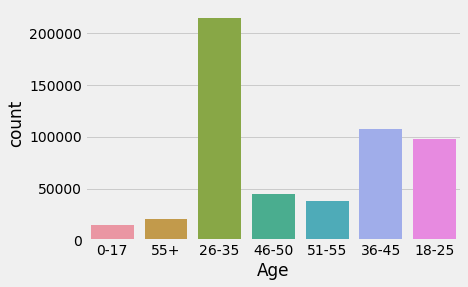
\includegraphics[width=0.3\textwidth]{ima/age_purchase.png}}
\frame{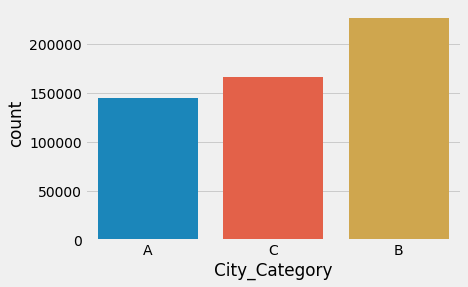
\includegraphics[width=0.3\textwidth]{ima/city_purchase.png}}
\frame{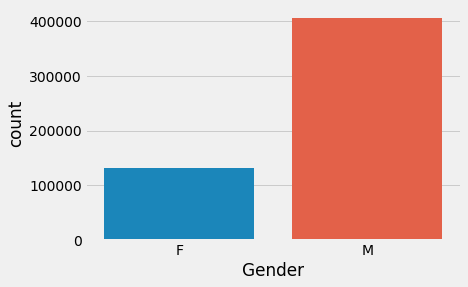
\includegraphics[width=0.3\textwidth]{ima/men_female_purchase.png}}
\frame{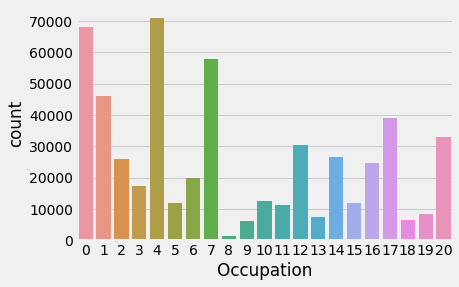
\includegraphics[width=0.3\textwidth]{ima/occupation_purchase.png}}
\frame{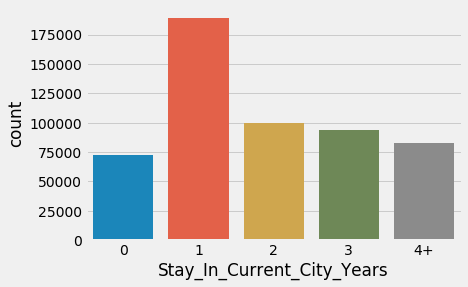
\includegraphics[width=0.3\textwidth]{ima/time_in_city_purchase.png}}
\frame{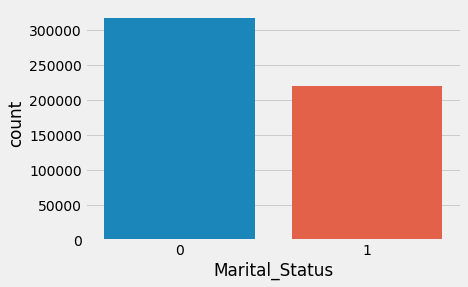
\includegraphics[width=0.3\textwidth]{ima/marital.png}}
%%\caption{...}
%%\abel{fig:...}
\end{figure}

Quest'analisi ci fornisce informazioni riguardo ai comportamenti sociali che questo tipo di eventi crea.

Analizzando ora rispetto alla variabile da stimare purchase si vede che:( vengono riportati solamente i dati rispetto alla stato civile, poiche i grafici non differiscono l'uno rispetto all'altro, inoltre possono essere visti nella citazione \cite{code} ).

\begin{figure}[htp!]
\centering
\frame{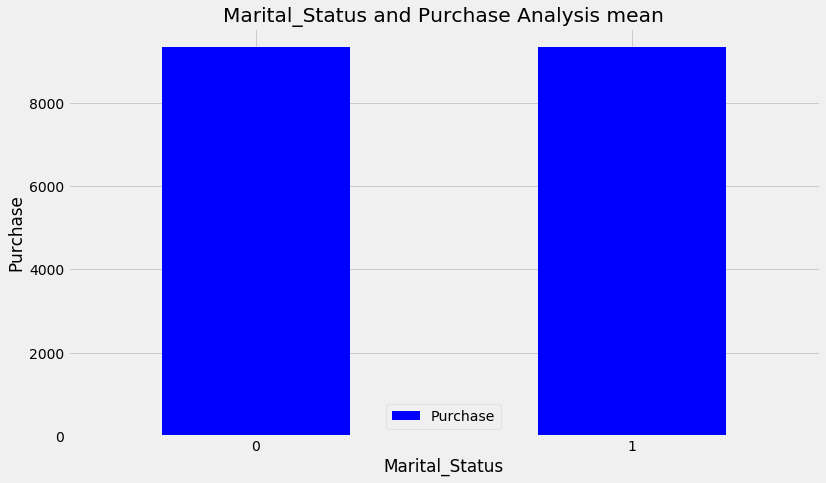
\includegraphics[width=0.3\textwidth]{ima/mean_marital_purc.png}}
\frame{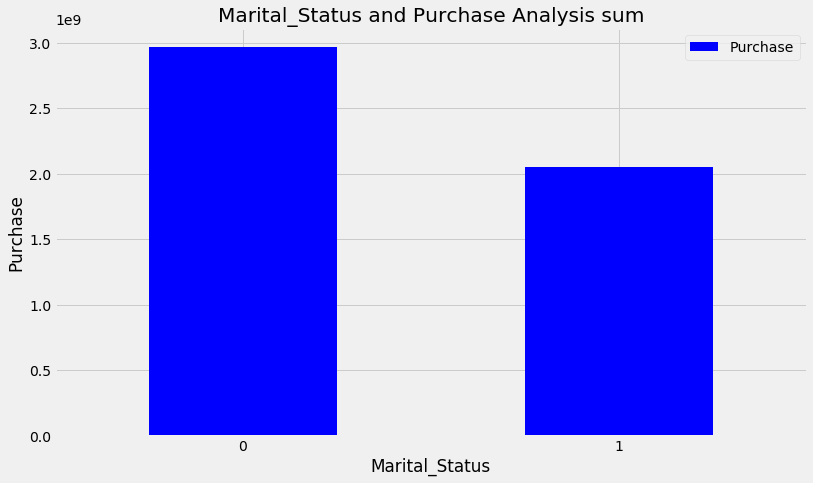
\includegraphics[width=0.3\textwidth]{ima/sum_marital.png}}
%%\caption{...}
%%\abel{fig:...}
\end{figure}

Dall'analisi dei grafici si vede che la media non fornisce informazioni utili a realizzare la predizione rispetto alle variabili note. L'informazione determinante risiede nella loro quantità perciò aggiungeremo come dato il volume per ogni categoria. cioè quantità: nome: Age\_ Count 	Occupation\_ Count 	Product\_ Category\_ 1\_ Count Product\_ Category\_ 2\_ Count 	Product\_ Category\_ 3\_ Count 	Product\_ ID\_ Count. 
Questa aggiunta ha permesso di avere una stima migliore rispetto al caso di eliminazione totale del dato, come evidenziato nella tabella 2.

Queste affermazioni non sono conducibili per quanto riguarda la categoria del prodotto come si vede nei  grafici 9-10:
\begin{figure}[htp!]
\centering
\frame{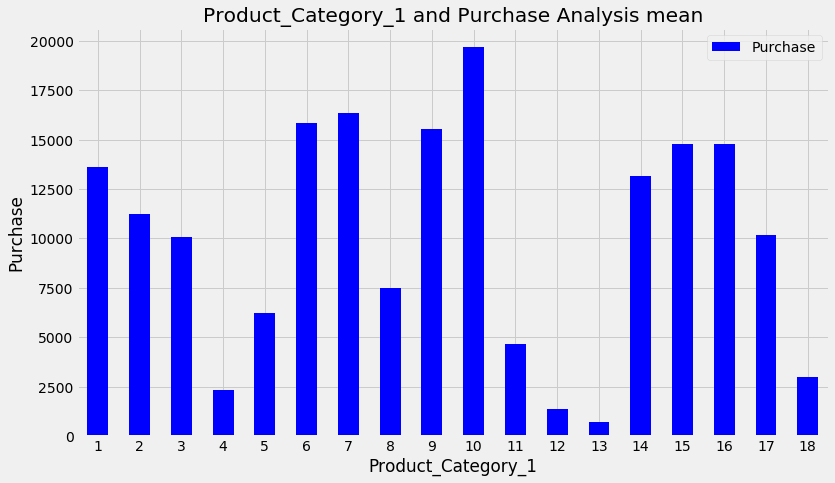
\includegraphics[width=0.3\textwidth]{ima/sum_cat_pur.png}}
\frame{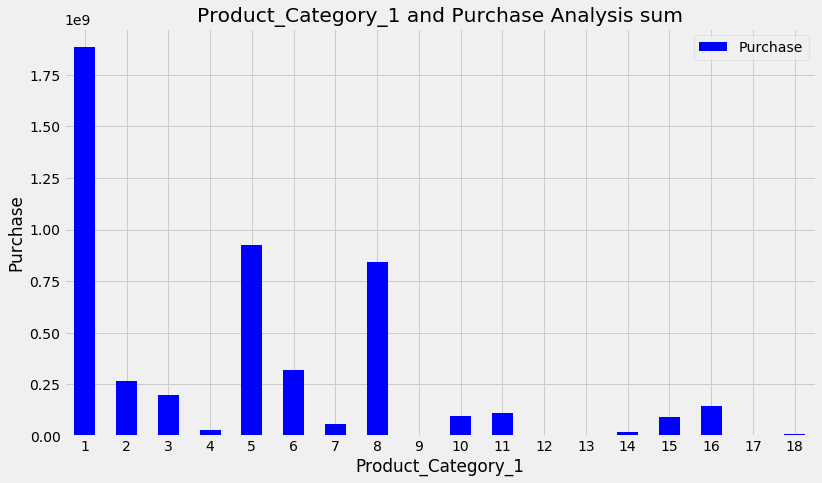
\includegraphics[width=0.3\textwidth]{ima/cate_purc.png}}
%%\caption{...}
%%\abel{fig:...}
\end{figure}

Analizzati i dati andremo a realizzare il modello:
 

\subsection{Procedimento}
Attualmente gli algoritmi gestiscono solo variabili di tipo numerico perciò abbiamo modificato la descrizione del dato dividentdolo ulteriormente in sottocategorie e assegnado uno 0 se non apparteneva a tale sottocategoria oppure un 1 se ci apparteneva.

qui sono riportati gli algoritmi scelti e le loro variabile, le altre variabili non elencate sono state scelte quelle di default delle librerie:
\begin{itemize}
\item linear regression : normalizzazione attiva;
\item DecisionTreeRegressor : max\_ depth=15, min\_ samples\_ leaf=100;
\item Random Forest: max\_ depth=8, min\_ samples\_ leaf=150.
\end{itemize}

mentre per la seconda:
\begin{itemize}
\item DecisionTreeRegressor : max\_ depth=15, min\_ samples\_ leaf=100;
\item Random Forest: max\_ depth=8, min\_ samples\_ leaf=150.
\end{itemize}

come descritto precedentemente abbiamo utilizzato i dati nel seguente modo:
il primo metodo utilizzato per predirre la quanti di soldi spesi è basato sull'eliminazione dei dati delle categorie dei prodotti 2 e 3, eliminando anche l'identificazione dell'utente perchè non influisce sulla predizione della spesa, così come il codice del prodotto.
Queste due ultime eliminazioni permettono di stimare meglio l'aggiunta di un nuovo utente però peggiorano la stima per un vecchio utente, dato che non c'è correlazione tra i suoi vecchi ordini. I risultati sono riportati nella prima tabella nella sezione risultati e discussione.

Il secondo metodo utilizza anche i dati della categoria 2 e 3 in più abbiamo anche tenuto conto delle rispettive quantità vendute e tenuto conto anche della quantità delle varie caratteristiche degli utenti, utilizzando tali dati abbiamo ottenuto una una stima migliore dato che aggiungo altre informazioni che descrivono i prodotti.

Utilizzando i dati nella struttura del secondo metodo ed eliminando ogni variabile legata al tipo di prodotto 'Product\_ ID', 'Product\_ Category\_ 2', 'Product\_ Category\_ 3','Product\_ Category\_ 1\_ Count', 'Product\_ Category\_ 2\_ Count', 'Product\_ Category\_ 3\_ Count', 'Product\_ ID\_ \_ Count'] abbiamo ottenuto i risultati riportati nella terza tabella:



\subsection{Risultati e discussione}
I risultati sono i seguenti:

Prima tabella:

\begin{tabular}{|p{0.2\textwidth}|p{0.2\textwidth}|p{0.2\textwidth}|p{0.2\textwidth}|}
\hline
Algoritmi &Linear Regression          & Decision tree regression         &random forest regression      \\
%\hline
%Risultati & 10.28\%            & 63.90\%     & 63.00\%          \\
\hline
RMSE (in dollari)     & 4708     & 2954                & 3008           \\
\hline
\end{tabular}

Seconda tabella:

\begin{tabular}{|p{0.2\textwidth}|p{0.1\textwidth}|p{0.2\textwidth}|p{0.2\textwidth}|}
\hline
Algoritmi &Linear Regression          & Decision Tree Regression         &Random Forest Regression      \\
%\hline
%Risultati &24.00\%            & 70.16\%    & 68.22\%          \\
\hline
RMSE (in dollari) &4344 &2685 &2802\\
\hline
\end{tabular}

come descritto in precedenza il migliore risultato sì è ottenuto modificando la struttura dei dati in modo da ottenere informazioni aggiuntive. Inoltre l'algorimo che meglio ha stimato è il Decision tree regression come evidenziato dal valore minimo di RMSE.

Terza tabella: 

\begin{tabular}{|p{0.2\textwidth}|p{0.2\textwidth}|p{0.2\textwidth}|p{0.2\textwidth}|}
\hline
%Algoritmi &Linear Regression          & Decision tree Classifier         &random forest Classifier      \\
%\hline
%Risultati & 10.71\%           & 86.79\%    & 82.72\%          \\
%\hline
%RMSE &3.552 &2.56 &2.807\\
Algoritmi          & Decision tree Classifier         &Random forest Classifier      \\
\hline
Risultati           & 86.79\%    & 82.72\%  \\
\hline
\end{tabular}

I risultati ottenuti hanno dimostrato che un modello Decision tree Classifier ha detrminato la miglior stima del tipo di categoria del prodotto.

\section{Conclusioni}
Il primi algoritmi ci hanno permesso di determinare che il decision tree regression con una gestione dei dati tenendo conto della loro rispettiva quantita ha fornito la miglior stima della variabile purchase.
mentre grazie alla struttura dei dati realizzata per il primo caso ci ha fornito un ottimo rislultato di stima della categoria. tale stima può esser eutilizzata come metodo per aumentare i profitti.
Un altro metodo per migliorare la stima sarebbe creare algoritmi ad och per ogni utente oppure un algorimo complessivo che tieene conto degli utenti. Il problema di questo tipo sarebbe l'aggiunta di un nuovo cliente e la pesantezza di molteplici algoritmi rispettivamente al contrario.
CIAO PAPA
GO FINI PER STA MATTINA

\nocite{*}
\printbibliography[title=Bibliografia]{}


\end{document}
